%\documentclass[10pt,ignorenonframetext,]{beamer}
\documentclass[hyperref={pdfpagemode=FullScreen},aspectratio=32]{beamer}
\usetheme{Darmstadt}
\setbeamertemplate{caption}[numbered]
\setbeamertemplate{caption label separator}{: }
\setbeamercolor{caption name}{fg=normal text.fg}
\usepackage{lmodern}
\usepackage{amssymb,amsmath}
\usepackage{ifxetex,ifluatex}
\usepackage{fixltx2e} % provides \textsubscript
\ifnum 0\ifxetex 1\fi\ifluatex 1\fi=0 % if pdftex
  \usepackage[T1]{fontenc}
  \usepackage[utf8]{inputenc}
\else % if luatex or xelatex
  \ifxetex
    \usepackage{mathspec}
  \else
    \usepackage{fontspec}
  \fi
  \defaultfontfeatures{Ligatures=TeX,Scale=MatchLowercase}
  \newcommand{\euro}{€}
\fi
% use upquote if available, for straight quotes in verbatim environments
\IfFileExists{upquote.sty}{\usepackage{upquote}}{}
% use microtype if available
\IfFileExists{microtype.sty}{%
\usepackage{microtype}
\UseMicrotypeSet[protrusion]{basicmath} % disable protrusion for tt fonts
}{}
\usepackage{color}
\usepackage{fancyvrb}
\newcommand{\VerbBar}{|}
\newcommand{\VERB}{\Verb[commandchars=\\\{\}]}
\DefineVerbatimEnvironment{Highlighting}{Verbatim}{commandchars=\\\{\}}
% Add ',fontsize=\small' for more characters per line
\usepackage{framed}
\definecolor{shadecolor}{RGB}{248,248,248}
\newenvironment{Shaded}{\begin{snugshade}}{\end{snugshade}}
\newcommand{\AlertTok}[1]{\textcolor[rgb]{0.94,0.16,0.16}{#1}}
\newcommand{\AnnotationTok}[1]{\textcolor[rgb]{0.56,0.35,0.01}{\textbf{\textit{#1}}}}
\newcommand{\AttributeTok}[1]{\textcolor[rgb]{0.77,0.63,0.00}{#1}}
\newcommand{\BaseNTok}[1]{\textcolor[rgb]{0.00,0.00,0.81}{#1}}
\newcommand{\BuiltInTok}[1]{#1}
\newcommand{\CharTok}[1]{\textcolor[rgb]{0.31,0.60,0.02}{#1}}
\newcommand{\CommentTok}[1]{\textcolor[rgb]{0.56,0.35,0.01}{\textit{#1}}}
\newcommand{\CommentVarTok}[1]{\textcolor[rgb]{0.56,0.35,0.01}{\textbf{\textit{#1}}}}
\newcommand{\ConstantTok}[1]{\textcolor[rgb]{0.00,0.00,0.00}{#1}}
\newcommand{\ControlFlowTok}[1]{\textcolor[rgb]{0.13,0.29,0.53}{\textbf{#1}}}
\newcommand{\DataTypeTok}[1]{\textcolor[rgb]{0.13,0.29,0.53}{#1}}
\newcommand{\DecValTok}[1]{\textcolor[rgb]{0.00,0.00,0.81}{#1}}
\newcommand{\DocumentationTok}[1]{\textcolor[rgb]{0.56,0.35,0.01}{\textbf{\textit{#1}}}}
\newcommand{\ErrorTok}[1]{\textcolor[rgb]{0.64,0.00,0.00}{\textbf{#1}}}
\newcommand{\ExtensionTok}[1]{#1}
\newcommand{\FloatTok}[1]{\textcolor[rgb]{0.00,0.00,0.81}{#1}}
\newcommand{\FunctionTok}[1]{\textcolor[rgb]{0.00,0.00,0.00}{#1}}
\newcommand{\ImportTok}[1]{#1}
\newcommand{\InformationTok}[1]{\textcolor[rgb]{0.56,0.35,0.01}{\textbf{\textit{#1}}}}
\newcommand{\KeywordTok}[1]{\textcolor[rgb]{0.13,0.29,0.53}{\textbf{#1}}}
\newcommand{\NormalTok}[1]{#1}
\newcommand{\OperatorTok}[1]{\textcolor[rgb]{0.81,0.36,0.00}{\textbf{#1}}}
\newcommand{\OtherTok}[1]{\textcolor[rgb]{0.56,0.35,0.01}{#1}}
\newcommand{\PreprocessorTok}[1]{\textcolor[rgb]{0.56,0.35,0.01}{\textit{#1}}}
\newcommand{\RegionMarkerTok}[1]{#1}
\newcommand{\SpecialCharTok}[1]{\textcolor[rgb]{0.00,0.00,0.00}{#1}}
\newcommand{\SpecialStringTok}[1]{\textcolor[rgb]{0.31,0.60,0.02}{#1}}
\newcommand{\StringTok}[1]{\textcolor[rgb]{0.31,0.60,0.02}{#1}}
\newcommand{\VariableTok}[1]{\textcolor[rgb]{0.00,0.00,0.00}{#1}}
\newcommand{\VerbatimStringTok}[1]{\textcolor[rgb]{0.31,0.60,0.02}{#1}}
\newcommand{\WarningTok}[1]{\textcolor[rgb]{0.56,0.35,0.01}{\textbf{\textit{#1}}}}
\usepackage{graphicx,grffile}
\makeatletter
\def\maxwidth{\ifdim\Gin@nat@width>\linewidth\linewidth\else\Gin@nat@width\fi}
\def\maxheight{\ifdim\Gin@nat@height>\textheight0.8\textheight\else\Gin@nat@height\fi}
\makeatother
% Scale images if necessary, so that they will not overflow the page
% margins by default, and it is still possible to overwrite the defaults
% using explicit options in \includegraphics[width, height, ...]{}
\setkeys{Gin}{width=\maxwidth,height=\maxheight,keepaspectratio}

% Comment these out if you don't want a slide with just the
% part/section/subsection/subsubsection title:
%\AtBeginPart{
%  \let\insertpartnumber\relax
%  \let\partname\relax
%  \frame{\partpage}
%}
%\AtBeginSection{
%  \let\insertsectionnumber\relax
%  \let\sectionname\relax
%  \frame{\sectionpage}
%}
%\AtBeginSubsection{
%  \let\insertsubsectionnumber\relax
%  \let\subsectionname\relax
%  \frame{\subsectionpage}
%}

\setlength{\emergencystretch}{3em}  % prevent overfull lines
\providecommand{\tightlist}{%
  \setlength{\itemsep}{0pt}\setlength{\parskip}{0pt}}
\setcounter{secnumdepth}{0}

\title{Estimating Demand and Supply}
\subtitle{Week 5 Slide Pack}
\author{Andrew Leach}
\date{}

\date[5/28/2017]
{\today}

%% Here's everything I added.
%%--------------------------

\usepackage{graphicx}
\usepackage{rotating}
%\setbeamertemplate{caption}[numbered]
\usepackage{hyperref}
\usepackage{caption}
\usepackage[normalem]{ulem}
%\mode<presentation>
\usepackage{wasysym}
\usepackage{tikz}
\usepackage{booktabs}
\usepackage{colortbl}
\usepackage{threeparttable}
\usepackage{dcolumn}
%\usepackage{amsmath}


\captionsetup{labelformat=empty}

% Get rid of navigation symbols.
%-------------------------------
\setbeamertemplate{navigation symbols}{}

% Optional institute tags and titlegraphic.
% Do feel free to change the titlegraphic if you don't want it as a Markdown field.
%----------------------------------------------------------------------------------


% \titlegraphic{\includegraphics[width=0.3\paperwidth]{\string~/Dropbox/teaching/clemson-academic.png}} % <-- if you want to know what this looks like without it as a Markdown field.
% -----------------------------------------------------------------------------------------------------


% Some additional title page adjustments.
%----------------------------------------
%\setbeamertemplate{title page}[empty]

\setbeamertemplate{title page}{%
  \vbox{}
%  \vfill
    \vspace{.5cm}% NEW
    \\
  \begingroup
    \centering
    \begin{beamercolorbox}[sep=8pt,center]{title}
      \usebeamerfont{title}BUEC 311: Business Economics, Organization
and Management\par%
        \vskip0.05em%
      \usebeamerfont{title}\inserttitle\par%
      \ifx\insertsubtitle\@empty%
      \else%
        \vskip0.5em%
        {\usebeamerfont{subtitle}\usebeamercolor[fg]{subtitle}\insertsubtitle\par}%
      \fi%
    \end{beamercolorbox}%
    \vskip1em\par
    \begin{beamercolorbox}[sep=4pt,center]{author}
      \usebeamerfont{author}\insertauthor
    \end{beamercolorbox}
    \vspace{0.5cm}% NEW
    \begin{beamercolorbox}[sep=8pt,center]{date}
      \usebeamerfont{date}\insertdate
    \end{beamercolorbox}\vskip0.05em
%    {\usebeamercolor[fg]{titlegraphic}\inserttitlegraphic\par}
  \endgroup
  %\vfill
}



%\date{}
\setbeamerfont{subtitle}{size=\large,shape=\scshape,series=\bfseries}
\setbeamerfont{title}{size=\Large,shape=\scshape,series=\bfseries}
\setbeamerfont{author}{size=\large}
\setbeamerfont{date}{size=\large}

\setbeamercovered{transparent}

% Some optional colors. Change or add as you see fit.
%---------------------------------------------------
 \definecolor{ualbertagreen}{HTML}{007C41}
\definecolor{ualbertagold}{HTML}{FFDB05}


% Some optional color adjustments to Beamer. Change as you see fit.
%------------------------------------------------------------------
\setbeamercolor{frametitle}{fg=ualbertagreen,bg=white}
\setbeamercolor{title}{fg=ualbertagreen,bg=white}
\setbeamercolor{author}{fg=ualbertagreen,bg=white}
\setbeamercolor{date}{fg=ualbertagreen,bg=white}
\setbeamercolor{local structure}{fg=ualbertagreen}
\setbeamercolor{section in toc}{fg=ualbertagreen,bg=white}
% \setbeamercolor{subsection in toc}{fg=ualbertagreen,bg=white}
\setbeamercolor{footline}{fg=ualbertagreen!50, bg=white}
\setbeamercolor{block title}{fg=ualbertagreen,bg=white}
\setbeamercolor{upper separation line head}{bg=ualbertagreen}
\setbeamercolor{lower separation line head}{bg=ualbertagold}
\setbeamercolor{middle separation line head}{bg=ualbertagold}
\setbeamercolor{frametitle}{fg=ualbertagreen,bg=white}

\setbeamercolor{section in head/foot}{bg=white,fg=ualbertagreen}
\setbeamercolor{author in head/foot}{bg=white,fg=ualbertagreen}
\setbeamercolor{date in head/foot}{bg=white,,fg=ualbertagreen}
\setbeamercolor{title in head/foot}{bg=white,fg=ualbertagreen}

\setbeamercolor{headline}{bg=white,fg=ualbertagreen}




\setbeamercolor*{middle separation line head}{bg=ualbertagreen}
\setbeamercolor*{alerted text}{fg=red}
\setbeamercolor*{example text}{fg=black}
\setbeamercolor*{structure}{fg=black}


\let\Tiny=\tiny


% Sections and subsections should not get their own damn slide.
%--------------------------------------------------------------
\AtBeginPart{}
\AtBeginSection{}
\AtBeginSubsection{}
\AtBeginSubsubsection{}

% Suppress some of Markdown's weird default vertical spacing.
%------------------------------------------------------------
\setlength{\emergencystretch}{0em}  % prevent overfull lines
\setlength{\parskip}{0pt}


\setbeamertemplate{headline}{%
\leavevmode%
%\ifnum\insertpagenumber>1
  \hbox{%
    \begin{beamercolorbox}[wd=\paperwidth,ht=5ex,dp=1.825ex]{white}%
    \usebeamerfont{headline}\hskip6ptBUEC 311: Estimating Demand and
Supply\par%
    \insertsectionnavigationhorizontal{\paperwidth}{}{\hskip0pt plus1filll}
    \end{beamercolorbox}%
  }
%\fi
}




% Allow for those simple two-tone footlines I like.
% Edit the colors as you see fit.
%--------------------------------------------------
\defbeamertemplate*{footline}{my footline}{%
    \ifnum\insertpagenumber=1
        \Tiny{%
            \hfill%
		\vspace*{1pt}%
            %\insertframenumber/\inserttotalframenumber \hspace*{0.1cm}%
            \newline%
            \color{ualbertagold}{\rule{\paperwidth}{0.4mm}}\newline%
            \color{ualbertagold}{\rule{\paperwidth}{.4mm}}%
        }
%    \hbox{%
%        \begin{beamercolorbox}[wd=\paperwidth,ht=.8ex,dp=1ex,center]{}%
%      % empty environment to raise height
%        \end{beamercolorbox}%
%    %}%
    %\vskip0pt%
    %no page number on the first page
    %    \Tiny{%
    %        \hfill%
   % 		\vspace*{1pt}%
    %        \color{ualbertagold}{\rule{\paperwidth}{0.4mm}}\newline%
    %        \color{ualbertagold}{\rule{\paperwidth}{.4mm}}%
%        }%
  \else%
        \Tiny{%
            \hfill%
		\vspace*{1pt}%
            \insertframenumber/\inserttotalframenumber \hspace*{0.1cm}%
            \newline%
            \color{ualbertagold}{\rule{\paperwidth}{0.4mm}}\newline%
            \color{ualbertagold}{\rule{\paperwidth}{.4mm}}%
        }%
    \fi%
}


% Various cosmetic things, though I must confess I forget what exactly these do and why I included them.
%-------------------------------------------------------------------------------------------------------
\setbeamercolor{structure}{fg=ualbertagreen}


\setbeamercolor{local structure}{parent=structure}
\setbeamercolor{item projected}{parent=item,use=item,fg=ualbertagreen,bg=white}
\setbeamercolor{enumerate item}{parent=item}

% Adjust some item elements. More cosmetic things.
%-------------------------------------------------
\setbeamertemplate{itemize item}{\color{ualbertagreen}$\bullet$}
\setbeamertemplate{itemize subitem}{\color{ualbertagreen}\scriptsize{$\bullet$}}
\setbeamertemplate{itemize/enumerate body end}{\vspace{.6\baselineskip}} % So I'm less inclined to use \medskip and \bigskip in Markdown.

% Automatically center images
% ---------------------------
% Note: this is for ![](image.png) images
% Use "fig.align = "center" for R chunks

% logo of my university
%\titlegraphic{
\includegraphics[width=3.5in]{UA-ASB-COLOUR.png}}
\logo{
\ifnum\insertpagenumber>1
   \tikz [remember picture,overlay]
    \node[yshift=.3cm,xshift=1.5cm] at (current page.south west)
        %or: (current page.center)
        {
\includegraphics[width=1in]{UA-ASB-COLOUR.png}};
        \fi
%
\includegraphics[height=0.8cm]{UA-ASB-COLOUR.png}\vspace{220pt}
}


\usepackage{etoolbox}

\AtBeginDocument{%
  \letcs\oig{@orig\string\includegraphics}%
  \renewcommand<>\includegraphics[2][]{%
    \only#3{%
      {\centering\oig[{#1}]{#2}\par}%
    }%
  }%
}

% I think I've moved to xelatex now. Here's some stuff for that.
% --------------------------------------------------------------
% I could customize/generalize this more but the truth is it works for my circumstances.

\ifxetex
\setbeamerfont{title}{family=\fontspec{serif}}
\setbeamerfont{frametitle}{family=\fontspec{serif}}
\usepackage[font=small,skip=0pt]{caption}
 \else
 \fi


% Okay, and begin the actual document...

\begin{document}
%%\frame{\titlepage}
%
\begin{frame}[plain]
   \tikz [remember picture,overlay]
    %\node[yshift=-0.5cm,xshift=0cm] at (current page.north)
        %or: (current page.center)
        \node[yshift=-0.75cm,xshift=2.5cm] at (current page.north west)
        %{
\includegraphics[width=3in]{UA-ASB-COLOUR.png}};
        {
\includegraphics[width=.35\paperwidth]{UA-ASB-COLOUR.png}}; \vspace{1cm}
   \titlepage
   \vfill
\end{frame}






\begin{frame}[fragile]
\begin{Shaded}
\begin{Highlighting}[]
\KeywordTok{library}\NormalTok{(rgl)}
\NormalTok{knitr}\OperatorTok{::}\NormalTok{knit\_hooks}\OperatorTok{$}\KeywordTok{set}\NormalTok{(}\DataTypeTok{webgl =}\NormalTok{ hook\_webgl)}


\NormalTok{utility\_map\textless{}{-}}\ControlFlowTok{function}\NormalTok{(x\_max,y\_max,u\_func,}\DataTypeTok{u\_vals=}\DecValTok{0}\NormalTok{,}\DataTypeTok{x\_shift=}\DecValTok{0}\NormalTok{,}\DataTypeTok{y\_shift=}\DecValTok{0}\NormalTok{,}
                      \DataTypeTok{x\_label=}\StringTok{"Consumption of Good X"}\NormalTok{,}
                      \DataTypeTok{y\_label=}\StringTok{"Consumption of Good Y"}
\NormalTok{                      )\{}

  \CommentTok{\#testing}
  \CommentTok{\# u\_func \textless{}{-} U}
  \CommentTok{\# u\_vals\textless{}{-}0}
  \CommentTok{\# x\_max=10}
  \CommentTok{\# y\_max=10}
  \CommentTok{\# x\_label="Consumption of Good X"}
  \CommentTok{\# y\_label="Consumption of Good Y"}
  \CommentTok{\# x\_shift=0}
  \CommentTok{\# y\_shift=0}
  \CommentTok{\# }

\CommentTok{\#build a grid}
\NormalTok{x\textless{}{-}}\StringTok{ }\KeywordTok{seq}\NormalTok{(}\DecValTok{0}\NormalTok{,x\_max,}\FloatTok{0.1}\NormalTok{)}
\NormalTok{y\textless{}{-}}\StringTok{ }\KeywordTok{seq}\NormalTok{(}\DecValTok{0}\NormalTok{,y\_max,}\FloatTok{0.1}\NormalTok{)}
  
  \CommentTok{\#populate it with z}
\NormalTok{  z\textless{}{-}}\KeywordTok{tibble}\NormalTok{()}
  \ControlFlowTok{for}\NormalTok{(x\_val }\ControlFlowTok{in}\NormalTok{ x)\{}
    \ControlFlowTok{for}\NormalTok{(y\_val }\ControlFlowTok{in}\NormalTok{ y)\{}
\NormalTok{      z\textless{}{-}}\KeywordTok{rbind}\NormalTok{(z,}\KeywordTok{tibble}\NormalTok{(x\_val,y\_val))}
\NormalTok{    \}}
\NormalTok{  \}}

\CommentTok{\#apply utility function}
\NormalTok{z\textless{}{-}z }\OperatorTok{\%\textgreater{}\%}\StringTok{ }\KeywordTok{mutate}\NormalTok{(}\DataTypeTok{z\_val=}\KeywordTok{u\_func}\NormalTok{(x\_val,y\_val))}


\CommentTok{\#do you want to populate some countours? Yes.}
\CommentTok{\#u\_vals=c(5,10,15)}

\CommentTok{\#if(u\_vals)}
\CommentTok{\#for(u in u\_vals)\{}
  \CommentTok{\#u\textless{}{-}5}
\CommentTok{\#  z\_cont\textless{}{-}z \%\textgreater{}\% filter(x\_val\textgreater{}0)\%\textgreater{}\%}
\CommentTok{\#    mutate(y\_val=contour\_solve(u\_func\_sent,u,x\_val))\%\textgreater{}\%}
\CommentTok{\#    mutate(z\_val=u\_func(x\_val,y\_val))}
\CommentTok{\#  z\textless{}{-}rbind(z,z\_cont)}
\CommentTok{\#  \}}



\CommentTok{\#find contour breaks}
\NormalTok{mult\_}\DecValTok{5}\NormalTok{\textless{}{-}}\KeywordTok{unique}\NormalTok{(z}\OperatorTok{$}\NormalTok{z\_val)[(}\KeywordTok{unique}\NormalTok{(z}\OperatorTok{$}\NormalTok{z\_val)}\OperatorTok{\%\%}\DecValTok{10}\OperatorTok{==}\DecValTok{0}\NormalTok{)]}
\CommentTok{\#n\_possibles\textless{}{-}length(mult\_5)}
\CommentTok{\#middle\textless{}{-}as.integer(n\_possibles/3)}
\CommentTok{\#middle2\textless{}{-}as.integer(2*n\_possibles/3)}
\NormalTok{contour\_breaks\textless{}{-}u\_vals}
\ControlFlowTok{if}\NormalTok{(u\_vals}\OperatorTok{==}\DecValTok{0}\NormalTok{)}
\NormalTok{  contour\_breaks\textless{}{-}mult\_}\DecValTok{5}


\CommentTok{\#graph the map}
\KeywordTok{ggplot}\NormalTok{(z)}\OperatorTok{+}
\StringTok{  }\KeywordTok{geom\_contour}\NormalTok{(}\KeywordTok{aes}\NormalTok{(x\_val,y\_val, }\DataTypeTok{z =}\NormalTok{ z\_val),}\DataTypeTok{breaks=}\NormalTok{contour\_breaks,}\DataTypeTok{size=}\FloatTok{1.5}\NormalTok{)}\OperatorTok{+}
\StringTok{  }\KeywordTok{geom\_dl}\NormalTok{(}\KeywordTok{aes}\NormalTok{(x\_val}\OperatorTok{+}\NormalTok{x\_shift,y\_val}\OperatorTok{+}\NormalTok{y\_shift, }\DataTypeTok{z =}\NormalTok{ z\_val,}\DataTypeTok{label=}\KeywordTok{paste}\NormalTok{(}\StringTok{"Utility="}\NormalTok{,}\KeywordTok{round}\NormalTok{(..level..,}\DecValTok{1}\NormalTok{))), }\DataTypeTok{method=}\StringTok{"bottom.pieces"}\NormalTok{, }
          \DataTypeTok{stat=}\StringTok{"contour"}\NormalTok{,}\DataTypeTok{breaks =}\NormalTok{contour\_breaks)}\OperatorTok{+}
\StringTok{  }\KeywordTok{class\_clean}\NormalTok{() }\OperatorTok{+}\StringTok{ }
\StringTok{  }\KeywordTok{coord\_equal}\NormalTok{()}\OperatorTok{+}
\StringTok{  }
\StringTok{  }\KeywordTok{theme}\NormalTok{(}\CommentTok{\#legend.position = "bottom",}
    \CommentTok{\#axis.text.x = element\_text(angle=90,hjust = .5,vjust=.5 ),}
    \DataTypeTok{panel.grid.major =}\KeywordTok{element\_line}\NormalTok{(}\DataTypeTok{colour =} \StringTok{"grey60"}\NormalTok{,}\DataTypeTok{linetype=}\StringTok{"dotted"}\NormalTok{,}\DataTypeTok{size=}\NormalTok{.}\DecValTok{5}\NormalTok{),}
    \CommentTok{\#panel.grid.minor =element\_line(colour = "black",linetype="dashed",size=.1),}
    \DataTypeTok{strip.text =} \KeywordTok{element\_text}\NormalTok{(}\DataTypeTok{size=}\KeywordTok{rel}\NormalTok{(.}\DecValTok{7}\NormalTok{) )}
\NormalTok{  )}\OperatorTok{+}
\StringTok{  }\CommentTok{\#annotate("text", x = as.Date(Sys.Date(){-}days(7)), y=0, label = "Last 14 days",size=1,hjust=0.5,vjust=0)+}
\StringTok{  }\KeywordTok{scale\_x\_continuous}\NormalTok{(}\DataTypeTok{breaks =} \KeywordTok{pretty\_breaks}\NormalTok{(),}\DataTypeTok{limits =} \KeywordTok{c}\NormalTok{(}\KeywordTok{min}\NormalTok{(x),}\KeywordTok{max}\NormalTok{(x)),}\DataTypeTok{expand =} \KeywordTok{c}\NormalTok{(}\DecValTok{0}\NormalTok{,}\DecValTok{0}\NormalTok{))}\OperatorTok{+}
\StringTok{  }\KeywordTok{scale\_y\_continuous}\NormalTok{(}\DataTypeTok{breaks =} \KeywordTok{pretty\_breaks}\NormalTok{(),}\DataTypeTok{limits =} \KeywordTok{c}\NormalTok{(}\KeywordTok{min}\NormalTok{(y),}\KeywordTok{max}\NormalTok{(y)),}\DataTypeTok{expand =} \KeywordTok{c}\NormalTok{(}\DecValTok{0}\NormalTok{,}\DecValTok{0}\NormalTok{))}\OperatorTok{+}
\StringTok{  }\KeywordTok{expand\_limits}\NormalTok{(}\DataTypeTok{y =} \DecValTok{0}\NormalTok{)}\OperatorTok{+}\StringTok{ }
\StringTok{  }\KeywordTok{scale\_colour\_manual}\NormalTok{(}\StringTok{""}\NormalTok{,}\DataTypeTok{values =} \KeywordTok{c}\NormalTok{(}\StringTok{"grey30"}\NormalTok{))}\OperatorTok{+}
\StringTok{  }\KeywordTok{scale\_fill\_manual}\NormalTok{(}\StringTok{""}\NormalTok{,}\DataTypeTok{values =} \KeywordTok{c}\NormalTok{(}\StringTok{"grey70"}\NormalTok{))}\OperatorTok{+}
\StringTok{  }\KeywordTok{scale\_shape\_manual}\NormalTok{(}\StringTok{""}\NormalTok{,}\DataTypeTok{values =} \KeywordTok{c}\NormalTok{(}\DecValTok{20}\NormalTok{))}\OperatorTok{+}
\StringTok{  }\KeywordTok{labs}\NormalTok{(}\DataTypeTok{y=}\NormalTok{y\_label,}\DataTypeTok{x=}\NormalTok{x\_label,}
       \CommentTok{\#title="Indifference map",}
       \CommentTok{\#subtitle= expression(Utility\textasciitilde{}"function"\textasciitilde{}is\textasciitilde{}U\textasciitilde{}"="\textasciitilde{}sqrt(XY)),}
       \CommentTok{\#caption="Source: Statistics Canada Table 32{-}10{-}0056{-}01, Balance sheet of the agricultural sector as at December 31st, graph by Andrew Leach",}
       \OtherTok{NULL}\NormalTok{)}
\NormalTok{\}}
\end{Highlighting}
\end{Shaded}
\end{frame}

\hypertarget{introduction}{%
\section{Introduction}\label{introduction}}

\begin{frame}[fragile]{Introduction}
\begin{Shaded}
\begin{Highlighting}[]
\NormalTok{U \textless{}{-}}\StringTok{ }\ControlFlowTok{function}\NormalTok{(x,y) (x}\OperatorTok{*}\NormalTok{y)}
\KeywordTok{utility\_map}\NormalTok{(}\DecValTok{5}\NormalTok{,}\DecValTok{5}\NormalTok{,U,}\DataTypeTok{u\_vals =} \KeywordTok{c}\NormalTok{(}\DecValTok{2}\NormalTok{,}\DecValTok{4}\NormalTok{,}\DecValTok{6}\NormalTok{,}\DecValTok{8}\NormalTok{,}\DecValTok{10}\NormalTok{),}\DataTypeTok{x\_shift =} \FloatTok{{-}.35}\NormalTok{,}\DataTypeTok{y\_shift =} \FloatTok{.25}\NormalTok{)}
\end{Highlighting}
\end{Shaded}

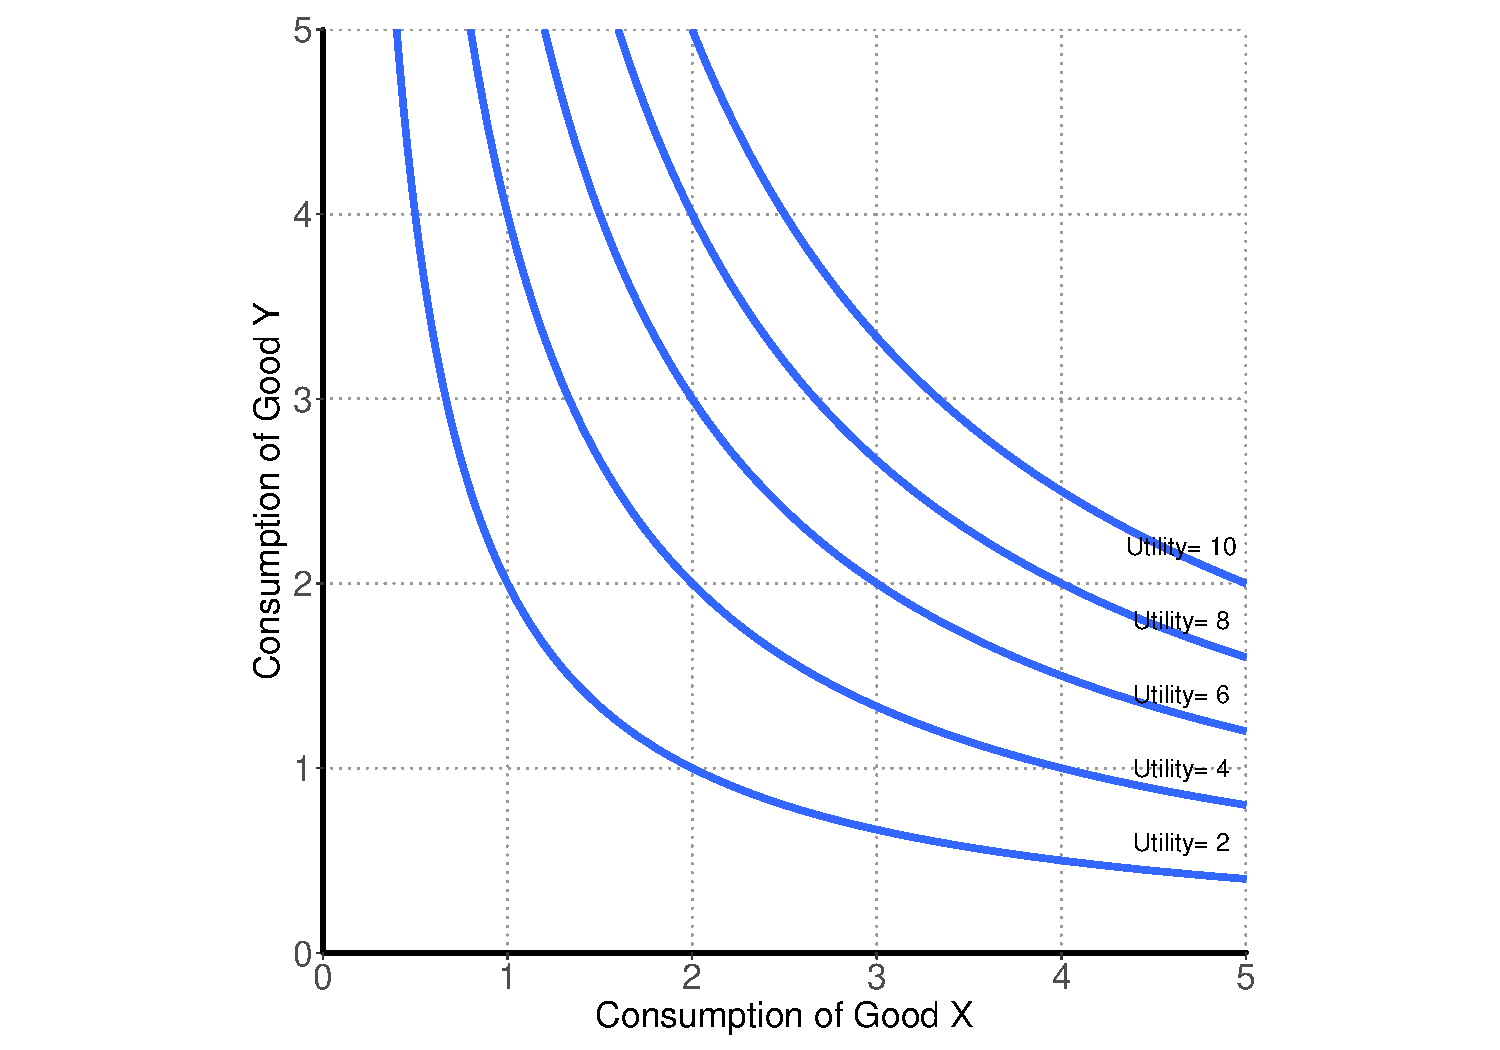
\includegraphics{utils_rgl_files/figure-beamer/making_graphs-1.pdf} \#
Introduction 2

\begin{Shaded}
\begin{Highlighting}[]
\NormalTok{x \textless{}{-}}\StringTok{ }\KeywordTok{sort}\NormalTok{(}\KeywordTok{rnorm}\NormalTok{(}\DecValTok{1000}\NormalTok{))}
\NormalTok{y \textless{}{-}}\StringTok{ }\KeywordTok{rnorm}\NormalTok{(}\DecValTok{1000}\NormalTok{)}
\NormalTok{z \textless{}{-}}\StringTok{ }\KeywordTok{rnorm}\NormalTok{(}\DecValTok{1000}\NormalTok{) }\OperatorTok{+}\StringTok{ }\KeywordTok{atan2}\NormalTok{(x,y)}
\KeywordTok{plot3d}\NormalTok{(x, y, z, }\DataTypeTok{col =} \KeywordTok{rainbow}\NormalTok{(}\DecValTok{1000}\NormalTok{))}
\end{Highlighting}
\end{Shaded}
\end{frame}


%\section[]{}
%\frame{\small \frametitle{Table of Contents}
%\tableofcontents}
\end{document}
